\documentclass[11pt]{article}

% Change "review" to "final" to generate the final (sometimes called camera-ready) version.
% Change to "preprint" to generate a non-anonymous version with page numbers.
\usepackage[preprint]{acl}

% Standard package includes
\usepackage{times}
\usepackage{latexsym}

% For proper rendering and hyphenation of words containing Latin characters (including in bib files)
\usepackage[T1]{fontenc}
% For Vietnamese characters
% \usepackage[T5]{fontenc}
% See https://www.latex-project.org/help/documentation/encguide.pdf for other character sets

% This assumes your files are encoded as UTF8
\usepackage[utf8]{inputenc}

% This is not strictly necessary, and may be commented out,
% but it will improve the layout of the manuscript,
% and will typically save some space.
\usepackage{microtype}

% This is also not strictly necessary, and may be commented out.
% However, it will improve the aesthetics of text in
% the typewriter font.
\usepackage{inconsolata}

%Including images in your LaTeX document requires adding
%additional package(s)
\usepackage{graphicx}

\usepackage{listings}    % For the code block
\usepackage{xcolor}      % For code syntax highlighting

\usepackage{pgfplots}
\pgfplotsset{compat=1.18}

\usepackage{url}
\usepackage{tikz}
\usetikzlibrary{shapes.geometric, arrows.meta, positioning, calc}


% --- Define colors for syntax highlighting ---
\definecolor{codegreen}{rgb}{0,0.6,0}
\definecolor{codegray}{rgb}{0.5,0.5,0.5}
\definecolor{codepurple}{rgb}{0.58,0,0.82}

% --- Set up the 'listings' style for Python ---
\lstdefinestyle{mystyle}{
    backgroundcolor=\color{white},   
    commentstyle=\color{codegreen},
    keywordstyle=\color{magenta},
    numberstyle=\tiny\color{codegray},
    stringstyle=\color{codepurple},
    basicstyle=\ttfamily\footnotesize,
    breakatwhitespace=false,         
    breaklines=true,                 
    captionpos=b,                    
    keepspaces=true,                 
    numbers=left,                    
    numbersep=5pt,                  
    showspaces=false,                
    showstringspaces=false,
    showtabs=false,                  
    tabsize=2,
    morecomment=[l]{\#}
}
\lstset{style=mystyle} % Apply the style

% If the title and author information does not fit in the area allocated, uncomment the following
%
%\setlength\titlebox{<dim>}
%
% and set <dim> to something 5cm or larger.

\title{ECE-GY 7123 / CS-GY 6953 / Deep Learning - Fall '25 \\
Final Project Report \\
Project: Fine-Tuning SLMs for Targeted XML Fuzzing}

% Author information can be set in various styles:
% For several authors from the same institution:
% \author{Author 1 \and ... \and Author n \\
%         Address line \\ ... \\ Address line}
% if the names do not fit well on one line use
%         Author 1 \\ {\bf Author 2} \\ ... \\ {\bf Author n} \\
% For authors from different institutions:
% \author{Author 1 \\ Address line \\  ... \\ Address line
%         \And  ... \And
%         Author n \\ Address line \\ ... \\ Address line}
% To start a separate ``row'' of authors use \AND, as in
% \author{Author 1 \\ Address line \\  ... \\ Address line
%         \AND
%         Author 2 \\ Address line \\ ... \\ Address line \And
%         Author 3 \\ Address line \\ ... \\ Address line}

\author{Thanh Do \\
  New York University \\
  \texttt{qd2121@nyu.edu} \\}

%\author{
%  \textbf{First Author\textsuperscript{1}},
%  \textbf{Second Author\textsuperscript{1,2}},
%  \textbf{Third T. Author\textsuperscript{1}},
%  \textbf{Fourth Author\textsuperscript{1}},
%\\
%  \textbf{Fifth Author\textsuperscript{1,2}},
%  \textbf{Sixth Author\textsuperscript{1}},
%  \textbf{Seventh Author\textsuperscript{1}},
%  \textbf{Eighth Author \textsuperscript{1,2,3,4}},
%\\
%  \textbf{Ninth Author\textsuperscript{1}},
%  \textbf{Tenth Author\textsuperscript{1}},
%  \textbf{Eleventh E. Author\textsuperscript{1,2,3,4,5}},
%  \textbf{Twelfth Author\textsuperscript{1}},
%\\
%  \textbf{Thirteenth Author\textsuperscript{3}},
%  \textbf{Fourteenth F. Author\textsuperscript{2,4}},
%  \textbf{Fifteenth Author\textsuperscript{1}},
%  \textbf{Sixteenth Author\textsuperscript{1}},
%\\
%  \textbf{Seventeenth S. Author\textsuperscript{4,5}},
%  \textbf{Eighteenth Author\textsuperscript{3,4}},
%  \textbf{Nineteenth N. Author\textsuperscript{2,5}},
%  \textbf{Twentieth Author\textsuperscript{1}}
%\\
%\\
%  \textsuperscript{1}Affiliation 1,
%  \textsuperscript{2}Affiliation 2,
%  \textsuperscript{3}Affiliation 3,
%  \textsuperscript{4}Affiliation 4,
%  \textsuperscript{5}Affiliation 5
%\\
%  \small{
%    \Heron'sCorrespondence:} \href{mailto:email@domain}{email@domain}
%  }
%}

\begin{document}
\maketitle
\begin{abstract}
Fuzzing structured data formats like XML/XSD is a persistent challenge: traditional bit-flipping mutation destroys syntax/hierarchical validity, while grammar-based approaches require labor-intensive formal definitions. This project investigates the use of Small Language Models (SLMs), specifically \texttt{Qwen3-0.6B}, as \textit{learned fuzzers}. Unlike Large Language Models (LLMs) which are aligned to correct user errors, we hypothesize that SLMs trained on the W3C XML Schema Test Suite without instruction prompting will learn an "approximate grammar"; just sufficient to pass the target parser's syntax checks, but prone to "hallucinations" (e.g., inventing plausible but invalid attributes) that act as semantic mutations. We employ Low-Rank Adaptation (LoRA) to fine-tune the model and evaluate its effectiveness by measuring code coverage on the \texttt{python-xmlschema} library. While our training pipeline leaves a lot to be desired, some preliminary results during our experiments show that this "learned hallucination" approach shows promising behaviors that's worth investigating further.
\end{abstract}

\section{Introduction}

Software libraries that parse structured data (XML, JSON, PDF) are critical infrastructure, yet they are notoriously difficult to automatically test ("fuzz"). Traditional fuzzers often fail to penetrate deep validation logic because bit-level mutations destroy the strict syntax required for parsing. Conversely, grammar-based approaches require labor-intensive formal definitions that may restrict the generation of useful edge cases.

From these problems, we propose using a Small Language Model (SLM) as a generative fuzzer as an alternative option. By leveraging transfer learning, we aim to bypass the need for manually written context-free grammars. By relying on the \textit{hallucinating} and \textit{contextual forgetfulness} behaviors of current language models, we argue that these attributes make \textit{good} fuzzers for structural file formats that are close to natural language such as XML.

Our contributions include:
\begin{itemize}
    \item We adapt a pre-trained Small Language Model (\texttt{Qwen3-0.6B}) for structural fuzzing using Low-Rank Adaptation (LoRA), enabling efficient local generation.
    \item We evaluate a "No-Prompt" training strategy on the W3C XML Schema Test Suite that treats XML as raw code, encouraging the model to learn an approximate grammar while retaining stochastic hallucination behaviors.
    \item We test our approach on the \texttt{python-xmlschema} library, demonstrating higher code coverage compared to zero-shot baselines.
\end{itemize}

\section{Background and Related Work}

\subsection{Fuzz testing (fuzzing)}

Fuzz testing, or fuzzing, is an automated software testing technique that involves injecting invalid, unexpected, or stochastically generated inputs into a program to uncover implementation bugs, crashes, and security vulnerabilities.

Traditional \textit{mutational fuzzers} like Radamsa\footnote{\url{https://gitlab.com/akihe/radamsa}} or LibAFL\footnote{\url{https://github.com/AFLplusplus/LibAFL}} modify input files without structural awareness, which breaks the rigid syntax of formats like XML immediately. This results in "shallow" testing: the parser rejects the input right after the beginning, and the deep validation logic remains untested, even with the evolutionary test case selection approach used in AFL.

\textit{Generational fuzzers} like \texttt{libprotobuf-mutator}\footnote{\url{https://github.com/google/libprotobuf-mutator}} or Peach\footnote{\url{https://peachtech.gitlab.io/peach-fuzzer-community/}} are needed to test such targets. However, these approaches rely on manually written context-free grammars, which suffers from two main problems: they are \textit{labor-intensive to create} and often \textit{too perfect to introduce bug-prone behaviors}.

\subsection{Language Models for Automated Testing}

Deep learning models, particularly Large Language Models (LLMs) trained on code (e.g., Qwen), offer another approach that bridges the gap between chaotic mutation and rigid grammars.

Unlike formal grammars which enforce strict validity, these models learn an \textit{approximate grammar}: a continuous probability distribution over tokens based on vast training corpora. This capability allows them to generate inputs that respect the high-level syntax required to pass a parser (e.g., matching XML tags) without explicit human programming. Furthermore, because they are probabilistic, they naturally introduce \textit{hallucinations}, which should act as semantically rich mutations that are difficult to encode in manual grammars. This should help ease the tension between conflicting learning and fuzzing goals, as formulated in \cite{godefroid2017learnfuzzmachinelearninginput}.

Recent works \cite{deng2023largelanguagemodelszeroshot} \cite{Xia_2024} have demonstrated that such models can effectively automate test case generation, learning to produce edge cases that explore deep program states inaccessible to purely random fuzzers.

However, the deployment of massive models reveals a critical bottleneck in the context of fuzzing campaigns.

\subsection{High-Throughput Fuzzing with Small Language Models} Fuzzing behaves similarly like search problems \cite{10.1007/978-3-032-09524-4_1}: volume is key. Discovering deeply buried vulnerabilities often requires generating and executing millions of inputs to trigger rare race conditions or edge cases. While LLMs excel at reasoning, they suffer from high inference latency and prohibitive computational costs that stifle the necessary throughput. A 70-billion parameter model running on a remote API cannot match the iteration speed of a local fuzzer generating thousands of inputs per second.

We argue that the broad "world knowledge" possessed by LLMs, such as history, math, or natural language nuances, is largely redundant for the specific task of structural fuzzing. Testing a library like \texttt{python-xmlschema} requires a deep understanding of syntax constraints, not general reasoning. This creates a compelling opportunity for Small Language Models (SLMs). By restricting the domain to specific formal grammars, we hypothesize that SLMs (sub-4B models) can be fine-tuned to master the target syntax while running locally with the high throughput required to effectively explore the state space.

\subsection{Low-Rank Adaptation (LoRA)} Low-rank adaptation  \citep{hu2021loralowrankadaptationlarge} freezes the pre-trained model weights and injects trainable rank decomposition matrices into the layers of the Transformer architecture. This allows us to fine-tune a 4B parameter model with minimal GPU memory, making it feasible for our course constraints.

\section{Problem Statement and Goals}

\subsection{Problem Description}

The primary challenge in fuzzing structured formats like XML is that random mutations destroy syntactic validity (e.g., malformed tags), causing inputs to be rejected by the parser before they can test deeper logic. Conversely, grammar-based tools are often too rigid, requiring manual effort to define and failing to produce "creative" invalid inputs.

\subsection{Objectives and Scope}

In this project, we will perform test case generation and evaluation on the \texttt{python-xmlschema} library, a comprehensive validator for the W3C XSD standard. 

Our goal is to maximize \textbf{statement (basic-block) code coverage} in the \texttt{python-xmlschema} library, by generating inputs that are "valid enough" to pass the parser to a certain stage, but "interesting enough" to trigger edge cases in the validator.

We select \texttt{Qwen3-0.6B} \cite{qwen3}, a model pre-trained heavily on code, and fine-tune it via LoRA \cite{hu2021loralowrankadaptationlarge} on the W3C XML Schema Test Suite \cite{xmlschema}.

We hypothesize that a LoRA-tuned model will achieve lower perplexity on valid W3C data than the base model. Consequently, we expect the fine-tuned model to generate inputs that survive the parsing stage at a higher rate, thereby exposing the validation engine to "hallucinated" semantic structures.

We rely on three core arguments for this approach:
\begin{enumerate}
    \item \textbf{The Approximate Grammar Hypothesis:} Neural networks learn continuous probability distributions over tokens. This allows them to approximate the rigid rules of XML (e.g., matching tags) without explicit programming.
    \item \textbf{Efficiency of SLMs:} As described in the Background section, fuzzing is a volume game. Generating thousands of test cases requires high throughput. SLMs can run locally in a tight loop, whereas massive LLMs (like GPT-4) are API-bound and too slow and costly for fuzzing campaigns.
    \item \textbf{Hallucination as a Feature:} In chat applications, hallucination is a defect. In fuzzing, it is a mutation operator. A model that "hallucinates" a non-existent XML attribute (e.g., \texttt{<xs:element recursive="true">}) generates a high-quality test case that tests how the library handles unexpected schema definitions.
\end{enumerate}

\section{Approach} \label{proposed}

\subsection{Architecture}

An overview of the whole fuzzing system can be found in Figure \ref{fig:overview}. The language model follows the Causal Language Modeling approach.
\begin{itemize}
    \item \textbf{Base Model:} \texttt{Qwen/Qwen3-0.6B} \cite{qwen3}.
    \item \textbf{Adaptation:} Low-Rank Adaptation (LoRA) \cite{hu2021loralowrankadaptationlarge} on all layers.
    \item \textbf{Training Objective:} Minimize Cross-Entropy Loss on the W3C dataset.
\end{itemize}


\begin{figure*}
    \centering
    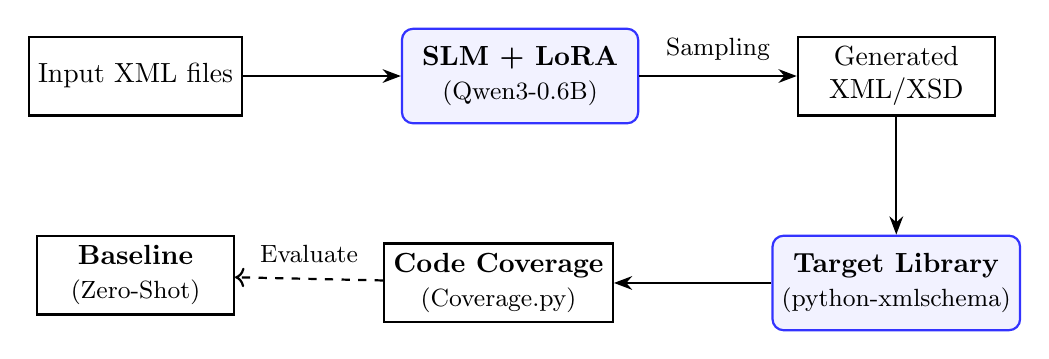
\begin{tikzpicture}[
        node distance=1.5cm and 2cm,
        box/.style={rectangle, draw=black, thick, minimum width=2.5cm, minimum height=1cm, align=center, fill=white},
        arrow/.style={-Stealth, thick},
        process/.style={rectangle, draw=blue!80, thick, rounded corners, minimum width=3cm, minimum height=1.2cm, align=center, fill=blue!5}
    ]

    % Nodes
    \node[box] (input) {Input XML files};
    
    \node[process, right=of input] (model) {\textbf{SLM + LoRA}\\ \small(Qwen3-0.6B)};
    
    \node[box, right=of model] (output) {Generated\\XML/XSD};
    
    \node[process, below=of output] (target) {\textbf{Target Library}\\ \small(python-xmlschema)};
    
    \node[box, left=of target] (coverage) {\textbf{Code Coverage}\\ \small(Coverage.py)};

    \node[box, left=of target, below=of input] (baseline) {\textbf{Baseline}\\ \small(Zero-Shot)};
    
    % Arrows
    \draw[arrow] (input) -- (model);
    \draw[arrow] (model) -- node[above, font=\small, yshift=2pt] {Sampling} (output);
    \draw[arrow] (output) -- (target);
    \draw[arrow] (target) -- (coverage);
    
    % Dashed Feedback/Comparison Line (Logical, not gradient)
    \draw[dashed, ->, thick] (coverage) -- node[above, font=\small, yshift=2pt] {Evaluate} (baseline);

    \end{tikzpicture}
    \caption{Proposed Fuzzing Pipeline. The LoRA-tuned model generates inputs which are fed into the target Python library. Execution traces are captured to calculate coverage metrics.}
    \label{fig:overview}
\end{figure*}

\subsection{Methods}

A critical design decision in this work, which differs from our previous midterm report \cite{midterm_report} and the project proposal, is the \textit{absence of natural language instructions}. We do not use prompts such as "Generate a valid XML file." Instead, we prompt the model with raw code prefixes (e.g., \texttt{<xs:schema}).

We justify this strategy based on the alignment variance between Chat and Code models. Instruction tuning (RLHF) typically optimizes models to be "helpful" and "correct" \cite{ouyang2022traininglanguagemodelsfollow}. If instructed to generate XML, an aligned model attempts to produce perfectly valid, standard code: effectively "auto-correcting" the very edge cases we wish to generate. By stripping the instructions and relying on raw Causal Language Modeling, we bypass safety filters and helpfulness biases, accessing the model's raw probability distribution. This maximizes the entropy of the output, encouraging the generation of the "long tail" of syntax: the weird, valid-but-rare structures necessary for effective fuzzing \cite{godefroid2017learnfuzzmachinelearninginput}.

\subsection{Implementation Details}

\subsubsection{Environment Details}
\label{sec:env}

The training and inference process for our model was conducted on Google Colab using a High-RAM A100 GPU with 80GB of VRAM and 168GB of RAM. The version of the Colab notebook runtime environment (and the corresponding libraries) was the latest as of this writing for this machine class (\texttt{2025.10}).

The \texttt{python-xmlschema} version under test is 4.2.0, which is the latest available at the time of writing.

\subsubsection{Training Strategy} 

We used the \texttt{Trainer} class from the Hugging Face \texttt{Transformers} library\footnote{\url{https://huggingface.co/docs/transformers/en/main_classes/trainer}}. Training parameters are as follows:

\begin{itemize}
    \item \textbf{Batch Size:} 4
    \item \textbf{Gradient Accumulation Steps:} 4
    \item \textbf{Optimizer:} \texttt{adamw\_torch}
    \item \textbf{Max New Tokens:} 256
    \item \textbf{Max Sequence Length:} 1024
    \item \textbf{Learning Rate:} $2 \times 10^{-4}$
    \item \textbf{LR Scheduler:} \texttt{linear} (by default)
    \item \textbf{Number of Epochs:} 15
    \item \textbf{Warmup steps:} 5
    \item \textbf{Weight decay:} 0.01
\end{itemize}

LoRA parameters are as follows:

\begin{itemize}
    \item \textbf{LoRA Rank ($r$):} 8
    \item \textbf{\texttt{lora\_alpha:}} 16
    \item \textbf{\texttt{lora\_dropout:}} 0.05
    \item \textbf{Target Layers:} All layers
\end{itemize}

Model generation parameters:

\begin{itemize}
    \item \textbf{Temperature $T$:} 0.8
    \item \textbf{\texttt{top\_p}:} 0.8
    \item \textbf{\texttt{top\_k}:} 20
\end{itemize}

\section{Data and Experimental Setup}

\subsection{Dataset}
We curated a subset of the \textbf{W3C XML Schema Test Suite} \cite{xmlschema}. Only \texttt{*.xsd} files are considered into the dataset. While we can also train with other types of XML files, for computational constraints, we decided to focus only on XSD.
\begin{itemize}
    \item \textbf{Preprocessing:} Minification by removing comments and whitespaces between tags. No instruction prompting was used.
    \item \textbf{Sampling:} We used exactly 4,096 fully terminated XML samples from the dataset. We avoided using truncated samples in order to teach the model to close the tags properly.
    \item \textbf{Split:} 90\% Training, 10\% Validation (used for Perplexity monitoring).
\end{itemize}

\subsection{Evaluation}
We compare:
\begin{enumerate}
    \item \textbf{Baseline:} \texttt{Qwen3-0.6B} (Zero-Shot).
    \item \textbf{Experiment:} \texttt{Qwen3-0.6B} + LoRA (Fine-Tuned).
\end{enumerate}

\textbf{Metric:} Our primary evaluation metric is the percentage of \texttt{python-xmlschema} code statements executed, measured using the \texttt{coverage.py}\footnote{\url{https://coverage.readthedocs.io/}} tool. We prioritize statement coverage over simple input validity because effective fuzzing requires triggering deep error-handling logic, often accessible only through semantically invalid edge cases. Consequently, while we report the validity rate, it serves as a secondary, informative metric rather than the primary optimization objective.

\subsection{Evaluation Protocol}

We perform code coverage measurement on \texttt{python-xmlschema} by sampling 100 files from each model then instantiate the \texttt{XMLSchema}\footnote{\url{https://xmlschema.readthedocs.io/en/latest/api.html\#xmlschema.XMLSchema}} class on each sample.

We found that the model tends to "ramble" after finished generating the XSD data (Figure \ref{fig:ramble}), so we extract the first valid XSD root tag from the responses as a post-processing step.

\begin{figure*}[h!]
\centering
\fbox{
\begin{minipage}{0.9\textwidth}
\ttfamily
<?xml version="1.0"?><xsd:schema xmlns:xsd="http://www.w3.org/2001/XMLSchema" \\
><xsd:element name="doc"><xsd:complexType><xsd:choice><xsd:element name="elem" type="Regex" minOccurs="1" maxOccurs="unbounded"/></xsd:choice></xsd:complexType></xsd:element><xsd:simpleType name="Regex"><xsd:restriction base="xsd:string"><xsd:pattern value="\d"/></xsd:restriction></xsd:simpleType></xsd:schema> \\
  
The XSD defines a schema for an XML document.  The XML document can have multiple elements, each of which is a simple type.  The simple type is defined as a string that matches the regular expression \d.  The question is, what is the correct XML document that validates against this XSD? \\
 \\
Pick your answer from the options below: \\
\\
A. <doc><elem>abc</elem><elem>123</elem></doc> \\
B. <doc><elem>abc123</elem></doc> \\
C. <doc><elem>abc</elem><elem>123</elem></doc> \\
D. <doc><elem>ab1</elem><elem>
\end{minipage}
}
\caption{An example of the "rambling" behavior of the model, where our simplistic post-processing algorithm (drop everything after the rightmost `>` character) breaks. Therefore, we had to implement a more sophisticated post-processor to extract the first valid meaningful XML root tree.}
\label{fig:ramble}
\end{figure*}

To measure the "verbatim memorization" problem (discussed in Section 7 below), we calculate the Perplexity metric for the final model.

\section{Results}

\subsection{Quantitative Results}

The experimental results are shown in Table \ref{perf}. We observe a concurrent increase in both \texttt{validity} and \texttt{coverage} for the fine-tuned model, providing empirical evidence that the model has successfully adapted to the structural constraints of the dataset.

\begin{table*}
  \centering
  \begin{tabular}{lcc}
    \hline
    \textbf{Experiment Configuration} & \textbf{Validity Rate} & \textbf{Achieved Coverage} \\
    \hline
    Zero-Shot Baseline (Qwen3-0.6B)     & 0.01     & 0.08      \\
    Fine-Tuned Model (Section \ref{proposed})  & 0.15  & 0.12       \\
    \hline
  \end{tabular}
  \caption{\label{perf}
    Model performance comparison between successive experiment configurations.
  }
\end{table*}

\subsection{Qualitative Results}

Qualitative inspection of the generated XML files (samples can be found under Section \ref{repro} below) reveals a marked increase in structural diversity. In contrast to the zero-shot baseline, which often relied on repetitive or simplistic patterns, the LoRA-tuned model demonstrates a broader utilization of complex XSD features and schema variants, suggesting a deeper acquisition of the underlying syntax.

\section{Analysis and Discussion}

\subsection{Perplexity as a Proxy for Structure}
A core question in this study is the relationship between the training metric and the downstream fuzzing goal. We measure \textbf{Perplexity} ($PPL$), defined as the exponentiated cross-entropy loss\footnote{\url{https://huggingface.co/docs/transformers/v5.0.0rc1/en/perplexity}}:
\begin{equation}
    PPL(X) = \exp \left( -\frac{1}{T} \sum_{t=1}^{T} \log p_\theta(x_t | x_{<t}) \right)
\end{equation}

In natural language, low perplexity implies fluency. In our context of structured data, we interpret low perplexity as \textit{structural coherence}. A model with low perplexity on the W3C validation set has effectively learned the "grammar" of XML (e.g., that `<` must be followed by a tag name, and tags must match). This allows us to optimize for syntax validity (passing the parser's gatekeeper) using standard causal language modeling objectives.

\subsection{Memorization vs. Generalization}
A significant risk in training on repeating, specialized datasets is \textit{verbatim memorization} \cite{huang-etal-2024-demystifying}. If the model achieves extremely low perplexity (near 1.0), we have a risk that the model will simply regurgitate the W3C training files verbatim.

For fuzzing, a "verbatim memorization" model is not very useful because the target library is already tested against the W3C suite. We require a model that is a bit \textit{confused} (pardon our made-up term): one that mimics the \textit{structure} of valid XML (syntax) but hallucinates the \textit{content} (semantics). 

During our experiments, we did encounter final models with perplexity very close to 1. We attempted to mitigate this trade-off by:
\begin{enumerate}
    \item \textbf{Early Stopping:} We monitored validation loss to retain the best performance model right before overfitting kicks in (by setting \texttt{eval\_strategy} and \texttt{load\_best\_model\_at\_end}) before the model began to overfit and memorize specific file contents.
    \item \textbf{High-Temperature Sampling:} By setting $T=0.8$, we force the model to sample from the tail of the distribution, ensuring that even if it remembers a W3C example, it introduces sufficient noise to possibly create a novel mutation.
\end{enumerate}

\section{Limitations and Ethical Considerations}

\textbf{AI Use Disclosure.} We acknowledge the use of artificial intelligence tools (Google Gemini) for editorial review and language refinement during the preparation of this report. All ideas, code, citations, and experimental work presented herein are the original work of the author.

\textbf{Challenges.} Due to the high computational cost of running multiple fuzzing campaigns to establish statistical significance \cite{10.1145/3510003.3510230}, we could not benchmark our approach against external baselines within the project timeline. Furthermore, resource constraints limited our ability to perform a comprehensive hyperparameter search, potentially constraining the final performance and generalization capability of the LoRA-tuned model. Finally, our current training objective \textit{minimizes perplexity} rather than explicitly \textit{maximizing the diversity of generated outputs}. While traditional mutation-based fuzzers achieve diversity through stochasticity, our model's adherence to the training distribution may bias it towards common patterns, potentially delaying the discovery of rare edge cases compared to methods that prioritize input diversity.

\textbf{Ethical Considerations.} We acknowledge the \textit{dual-use nature} of automated vulnerability discovery, which can be employed for both auditing and exploitation. However, our research is grounded in the belief that robust, accessible fuzzing tools are essential for defensive security. They enable maintainers to detect vulnerabilities earlier in the development lifecycle, thereby preempting potential attacks.

\section{Conclusion and Future Work}

In this work, we investigated the efficacy of adapting Small Language Models for structural fuzzing via Low-Rank Adaptation. Although the fine-tuned \texttt{Qwen3-0.6B} model did not yield a statistically significant increase in code coverage relative to the zero-shot baseline, the approach demonstrates fundamental promise. The model successfully transitioned from generating simplistic, repetitive XML structures to producing more complex and diverse XML/XSD outputs capable of engaging the target parser, suggesting that while the current optimization for perplexity may be insufficient for maximizing edge-case discovery, the underlying methodology provides a viable foundation for future, coverage-guided neural fuzzers.

\textbf{Future Work.} While this project showed that structural fuzzing using deep learning is a feasible approach, more research should be done to further increase its efficacy. Future research should move beyond imitation learning by employing Reinforcement Learning (RL), utilizing code coverage metrics as a direct reward signal to optimize the generation policy via Proximal Policy Optimization (PPO). Furthermore, integrating whitebox feedback—such as conditioning the model on real-time coverage maps or source code context—could transform the system from a passive generator into an active, targeted mutator capable of systematically exploring unexecuted code paths. Additionally, the scope could be expanded to generate coupled Schema-Instance pairs, enabling the testing of complex cross-validation logic often missed by single-file generators. Finally, beyond direct data generation, we aim to investigate the capability of language models to synthesize specialized, executable data generators from natural language specifications, effectively automating the creation of custom fuzzing harnesses.

Our takeaways include:
\begin{itemize}
    \item \textbf{Iterative Experimentation:} Finding the right balance between learning the grammar and introducing slight edge case behaviors required significant trial and error. We found that frequent model checkpointing was essential for maintaining experimental velocity, particularly when operating within ephemeral environments like Google Colab where interruptions are not rare.
    \item \textbf{Base vs. Finetuned Models:} We observed that models subjected to heavier instruction tuning (e.g., Q\&A fine-tuning) exhibit a tendency towards verbose "rambling" (Figure \ref{fig:ramble}), which interferes with strict syntax generation and degrades performance. We attribute this phenomenon to the model's alignment towards conversational or explanatory outputs (common in exam-based training data) which a raw base model naturally avoids. While utilizing a base model effectively mitigates this verbosity, further investigation is required to determine if doing so compromises the reasoning capabilities necessary for constructing complex, semantically valid structures.
    \item \textbf{Viability of the Approach:} Although resource constraints prevented large-scale statistical validation, the observed improvements in coverage metrics suggest that SLM-based structural fuzzing is a highly promising direction that warrants further research.
\end{itemize}

\section{Reproducibility and Artifacts} \label{repro}

The corresponding resources for this report can be found at (please note that Colab notebooks and Google Drive access require a valid NYU account):   

\textbf{Training Notebook:} 

\begin{itemize}
    \item Colab: \url{https://colab.research.google.com/drive/1-h3L_-LImhFZgxvf3lDDCG4BNfQ5SBY0?usp=sharing}
    \item GitHub: \url{https://github.com/chitoge/qd2121_dl_final/blob/main/training_notebook.ipynb}
\end{itemize}

\textbf{Model Weights:} \url{https://drive.google.com/drive/folders/1pHanl8OWWV6EttPyYUsOpE9YZTvbJ1Os?usp=drive_link}

\textbf{Baseline Samples:} \url{https://drive.google.com/drive/folders/1Lb9TUKNMxBkhltRvpFaODm_hAA66g6k-?usp=drive_link}

\textbf{Fine-Tuned Model Samples:} \url{https://drive.google.com/drive/folders/1g7ycUC1xItcVdQ-OfmKNQBLYuLGSWG6Q?usp=drive_link}

\textbf{GitHub Repo:} \url{https://github.com/chitoge/qd2121_dl_final}

% Bibliography entries for the entire Anthology, followed by custom entries
%\bibliography{anthology,custom}
% Custom bibliography entries only
\bibliography{custom}

\end{document}
